\documentclass[]{article}
\usepackage{ctex}
%opening
\usepackage{xcolor}
\usepackage{hyperref}
\usepackage{graphicx}
\usepackage{xcolor}
\usepackage{listings}
\title{}
\author{}


\definecolor{mycolor}{RGB}{255,0,255}
\lstset{
	language=Python,
	breaklines=true, % 允许自动换行
	breakatwhitespace=true, % 在空白处换行
}
\begin{document}
	% TODO: \usepackage{graphicx} required
	\maketitle
	\tableofcontents \newpage
	\section{Text\_To\_Speech函数}
\lstset{
	basicstyle=\ttfamily\small, % 使用较小的字体
	keywordstyle=\color{blue},
	language=Python,
	breaklines=true, % 自动换行
	frame=single,
	showstringspaces=false,
	postbreak=\mbox{\textcolor{red}{$\hookrightarrow$}\space} % 换行后的标记
}


	
	\subsection{函数概述}
	
	\texttt{text2speech} 函数用于将文本转换为语音,并播放或保存为 WAV 文件。该函数支持中断检测、异步播放和音量调整等功能。
	
	\subsection{参数说明}
	
	\begin{itemize}
		\item \texttt{text=''}: 待转换的文本,默认为空字符串。
		\item \texttt{index=0}:\\
		Index=1000表示同步播放,先文本转语音,然后在运行到播放语音的那一行代码时,会阻塞在那一行代码,直到语音全部播完,才会继续运行后面的代码\\
		Index=0表示异步播放,先文本转语音,然后在运行到播放语音的那一行代码时,会新开一个进程用来播音,而主程序可以继续推进,去对下一句话进行文本转语音,因此上一句话的播音和下一句话的文本转语音是同时进行的,节省时间\\
		值得注意的是,上一句话播音的进程会被记录到STATUS.LastPlayProcessor变量,一旦检测到打断,就会杀死上一句话播音的进程,防止用户打断之后,机器人还一直播音不停下
		\item \texttt{is\_beep=False}:\\is\_beep表示现在要播音的这句话是不是过渡句
		过渡句例如: “我在”、 “大家有什么问题吗”
		在播音的同时,会把正在播音的这句话记录到
		STATUS.LAST\_BROAD\_WORDS变量,日志中会记
		录这句话,以及用户听到这句话之后,用户说的下一
		句话,用途是测试语音识别的准确性\\
		例如日志中可能会记录:\\
		时间: yyyy.mm.dd, hh:mm:ss\\
		上一句播音的话:玉兔号是我国的月球探测车
		语音识别结果:玉兔号是什么时候登上月球的?
		由于过渡句中不包含信息,记录日志时不能仅仅记录
		过渡句,还应该把上上句播音的话也记录下来
		例如,当最后一句播音的话是过渡句,日志中可能会
		记录:\\
		时间: yyyy.mm.dd, hh:mm:ss\\
		上一句播音的话:这就是我对航天机械臂的介绍。\\
		大家有什么问题吗\\
		语音识别结果:航天机械臂有多长?\\
		此处“这就是我对航天机械臂的介绍。 ”就是上上句播
		音的话,由于最后一句播音的话是过渡句,所以上上
		句播音的话也会被记录在日志里
		\item \texttt{wavfile=None}: 指定 WAV 文件路径,若提供,则直接播放该文件而不进行文本到语音的转换。
		\item \texttt{ignore\_interrupt=False}: 是否忽略中断,默认为 False。若为 True,则即使检测到中断也继续播放。
	\end{itemize}
	
	\subsection{功能描述}
	
	\begin{enumerate}
		\item 检查音频输出设备是否存在,若不存在则打印提示信息并返回。
		\item 若未指定 \texttt{wavfile},则调用外部脚本进行文本到语音的转换,并保存为 WAV 文件。
		\item 检查是否有上一次的播放进程,若存在且未完成,则根据 \texttt{ignore\_interrupt} 参数决定是否中断上一次的播放。
		\item 调整生成的 WAV 文件的音量,并保存为新的文件。
		\item 根据音频卡的 ID,选择合适的播放方式进行播放。
		\item 根据 \texttt{index} 参数,决定是进行同步播放还是异步播放。
	\end{enumerate}
	
	\subsection{注意事项}
	
	\begin{itemize}
		\item 该函数依赖外部脚本和 \texttt{ffmpeg} 工具进行文本到语音的转换和音量调整。
		\item 要用进程自带的kill方法而非直接kill命令来终止正在进行的播放,防止播音卡死。
		\item 异步播放时,需要留出短暂的时间间隔,以避免文件读写冲突。
	\end{itemize}

\subsection{执行过程的没理解的地方}
\begin{itemize}
	\item 
	\begin{lstlisting}[language=Python]
ttsproc=subprocess.Popen(["python3","/home/kuavo/catkin_dt/
src/voice_pkg/scripts/kedaxunfei_tts/test_host_3090_tts.py", text, savepath])
\end{lstlisting}这个文件运行起来什么功能?\\答:tts是text\_to\_speech的缩写,不必深究内容。
	\item ttsproc.poll()有什么功能(已解决)?\\答:在Python中,poll()方法是subprocess.Popen对象的一个方法,用于检查子进程是否已经结束。如果子进程已经结束,poll()会返回子进程的退出码,这通常是一个整数值;如果子进程尚未结束,poll()会返回None。
	\item playproc,ttsproc,STATUS.Last\_Play\_Processor都是干什么的,什么时候要注意'在连续播放多次时,需要注意资源的释放和进程的管理,避免服务卡死。'\\答:\textbf{假设text2speech函数正要播放一句话text:
	ttsproc 是用来把text文本转为语音(即合成音频文件)的进程
	playproc 是用来把音频文件播放出来的进程\\
	STATUS.Last\_Play\_Processor 是上一句话播音的进程
	为什么要记录这些进程?因为一旦识别到用户的打断信号,此时
	正在进行的一切 文本转语音 和 播音 进程都应该被杀死。 只有
	把这些进程全部都记录下来,在识别到用户的打断信号时, 才能
	把它们全都杀死}
\end{itemize}	
	\section{listenuser}
	\subsection{函数描述}
	
	\texttt{listenuser} 函数用于根据用户的声音输入或键盘输入来获取用户的指令或信息。该函数支持通过声音输入和文本输入两种方式。当系统检测到声音输入设备时,会通过声音识别接口获取用户的指令;若未检测到声音输入设备,则会提示用户通过键盘输入信息。
	\subsection{参数说明}
	\begin{itemize}
		\item \textbf{text} (默认值: \texttt{'ding'}): 预设的文本输入,用于声音识别接口的默认输入。
		\item \textbf{iter} (默认值: \texttt{1}): 指定声音识别过程中的迭代次数,用于控制识别的精度或尝试次数。
	\end{itemize}
	\subsection{不确定的地方}
\begin{itemize}
	\item \textbf{ iat\_web\_api是做什么的,参数什么意思?}\\
	这个iat是用于语音识别的,就是语音转文本(Intelligent Audio Transcription)
	\item \textbf{ding有什么特殊的含义吗?}\\
	ding是提示音,提醒用户录音开始了。
	
\end{itemize}
\section{Pardon}

\texttt{pardon} 函数的目的是反复录制用户语音,直到获取到非空的语音输入为止,最多重复指定的轮数 \texttt{pardon\_round}。该函数在录制过程中提供了用户交互的反馈,并处理了用户可能的打断行为。

\subsection{参数说明}
\begin{itemize}
	\item \textbf{pardon\_round} (默认值: 1): 指定在放弃之前尝试录制用户语音的最大轮数。
\end{itemize}

\subsection{功能描述}
\begin{enumerate}
	\item 函数开始时,会打印一条消息提示开始录制用户语音。
	\item 通过 \texttt{listenuser} 函数反复录制用户语音,直到录制到非空的语音输入或达到最大重试次数。
	\item 如果录制到的语音为特定标记('\#\#\#\#'),或者是第一次提示用户提问,则通过 \texttt{text2speech} 函数反馈给用户,提示他们现在可以提问,并记录提示次数。
	\item 如果用户在6秒内没有说话,则会再次使用 \texttt{text2speech} 函数提示用户可以提问。
	\item 在用户提问过程中,如果检测到打断行为,会暂停QA(Question Answering)状态,并通过 \texttt{text2speech} 函数处理打断后的用户交互。
	\item 最后,无论是否录到有效语音,都会重置QA状态和打断状态,准备下一次录音或交互。
\end{enumerate}

\subsection{注意事项}
\begin{itemize}
	\item 该函数依赖于全局状态对象 \texttt{STATUS} 来管理QA状态和打断状态。
	\item 使用了 \texttt{listenuser} 和 \texttt{text2speech} 两个外部函数来分别处理语音输入和输出。
	\item 特殊标记 '\#\#\#\#' 用于特定逻辑处理,例如用户超时未回应时的处理。
\end{itemize}
\subsection{不理解的地方}
\begin{itemize}
	\item 用户超过 6 秒没有说话就询问一遍在代码里哪里体现?\\
	\textbf{listener那个函数的接口里有录音10秒左右,也就是等待时间了。}
	\item \#\#\#\#是代填充的唤醒词吗?\\
	\textbf{可以理解为唤醒词的标志}
	\item QAING这个状态有什么作用?\\
\textbf{	qaing的意思是正在qa(问答),如果set为True,那么将不会处理打断的信号。可以理解为一个linux里面的信号锁}
	\item 最后一个else是处理什么情况的?\\
\textbf{	就是没录到东西并且repeat count不是0的时候才会进入第三个分支,等待被打断,机器人说完提示词10秒内不回答,机器人就会卡在这等待人再用唤醒词(打断词)唤醒它}
\end{itemize}
	\section{QAClass}
	
	\texttt{QAClass} 是一个负责处理问答流程的类,它通过多线程初始化问答模型,并处理用户的提问,返回相应的答案。
	
	\subsection{构造函数}
	构造函数初始化了一个线程来启动问答模型的初始化过程,并设置了一些基本属性,如中断流的标志和任务类型标签列表。
	
	\subsection{QAClassInit}
	\texttt{QAClassInit} 方法用于初始化问答模型。它通过调用 \texttt{get\_llm\_answer} 函数获取模型实例,并将其存储在类的属性中。
	
	\subsection{answer\_question}
	\texttt{answer\_question} 方法是类的核心功能,负责处理用户的提问并返回答案。它首先等待问答模型初始化完成,然后根据用户的提问和其他相关信息,通过问答模型生成答案。此方法还处理了流式返回的答案,并在适当的时候通过语音合成技术将答案转换为语音输出。
	
	\subsection{\underline{我不理解的地方}}
\begin{itemize}
	\item \texttt{STATUS} 和 \texttt{get\_llm\_answer} 函数的具体实现和作用。(还包括 \texttt{llmclass} 的 \texttt{if\_document\_searched}, \texttt{process\_query} 这些)
	\item {mycolor}{self.llmclass.process\_query这个函数的返回结果是什么格式,有什么样例吗?流式和非流式的方式中,回答都是一次产生的,但是流式返回是按半句话来读,还能用非阻塞的方式节省时间,非流式是一次读完全部的回答是这个意思吗?}\\
	\textbf{答:} self.llmclass.process\_query 函数传入的是用户的问题,返回的是大模型生成的回答。分为非流式和流式两种情况。非流式就是最简单的情况,直接把大模型的回答完整返回,那么 self.llmclass.process\_query 函数的返回值就是一个字符串。流式是指一个字一个字返回,因为自回归生成式模型就是一个字一个字生成的,那么这样返回就会更快,不必等待回答完整生成才返回。此时 self.llmclass.process\_query 函数的返回值就不是字符串了,而是一个生成器,可以了解一下 python 的生成器,并在代码中搜索 yield 来看看生成器的用法。
	\item 816行,\texttt{text2speech("?")},这个问号怎么也能转语音\\
	\textbf{是为了保证打断,因为我们的打断是上一句.前面都是异步播放,本句后面没有下一句的话,播放过程不会被打断因此得手动加一句话。}
	\item \texttt{interrupt\_stream} 和 \texttt{STATUS} 里的 \texttt{interrupt} 什么区别,为什么要加上这个?
	\begin{itemize}
		\item \texttt{STATUS.is\_interrupted}\\
		\textbf{答:}
		
		\texttt{STATUS.is\_interrupted} 就是指用户有没有用唤醒词打断机器人,这个变量在整个流程中都非常重要。
		
		\item \texttt{self.interrupt\_stream}
		
		我们假设用户提出了问题,大模型正在流式生成回答并且播音。
		
		\begin{enumerate}
			\item 如果此时用户打断了机器人,那么就会立刻切断对大模型流式生成回答的播音,然后播放提示语“我在”或“大家有什么问题吗”。
			\item 如果用户从始至终都没有打断,那么就会把大模型生成的回答全部播放完毕。
		\end{enumerate}
		
		由于我们让大模型在回答问题时,最后几句话要引导用户继续下达指令,所以效果是这样的:比如用户提出问题,大模型的回答可能是:“......以上就是天宫二号的发射过程,您还有其他关于空间实验室的问题吗?”或者“......长征二号的故事我讲完了,如果您还对其他火箭感兴趣,可以让我带您参观运载火箭展区”,如此一来,就不需要再播放“我在”或“大家有什么问题吗”这类提示语。
		
		因此 \texttt{self.interrupt\_stream} 的含义是大模型生成的回答是否被完整播放完。
		
		而 \texttt{self.interrupt\_stream} 的作用是控制提示语的播放:如果大模型生成的回答没有被播放完,而是被打断了,那么 \texttt{self.interrupt\_stream} 为 \texttt{True},需要播放提示语;如果大模型生成的回答被完整播完了,没有被打断,那么大模型会自己生成一些引导用户提问的话,其作用相当于提示语,此时 \texttt{self.interrupt\_stream} 为 \texttt{False},不需要播放我们写死的提示语。
	\end{itemize}
	\item 853行 \texttt{if self.interrupt\_stream:}\\
	\texttt{sleep(0.05)}\\
	\texttt{STATUS.set\_is\_Interrupted(False)}\\
	\textbf{依旧没看明白,为什么等了0.05秒就给这个状态消除了,受到打断产生interrupt\_stream这个信号为什么只需要维持0.05秒?}\\
\textbf{答:} 这是一个历史遗留问题。首先需要明确的是,当用户使用唤醒词打断后,会在唤醒词回调函数中把 \texttt{STATUS.is\_Interrupted} 变量置为 \texttt{True}(可以了解一下什么是回调函数,具体的代码详见 \texttt{MainClass} 的 \texttt{def ivw\_callback()}),那么就一定需要在某个地方把这个变量重新恢复为 \texttt{False},也就是恢复为正常状态。

\hspace{2em} 853 行开始的这 3 行代码的含义是,如果用户使用唤醒词打断了大模型的回答播音(此时 \texttt{STATUS.is\_Interrupted} 变量已经自动变为 \texttt{True}),那么就在 0.05 秒后,把这个变量重新恢复为 \texttt{False},中间留的 0.05 秒是为了给其他程序反应时间(例如打断播音的程序),其他程序会在 \texttt{while} 循环中不停检测 \texttt{STATUS.is\_Interrupted} 变量,留出 0.05 秒防止其他程序还没有检测到打断,这个变量就被恢复了。

\hspace{2em} 可以看到 \texttt{answer\_question} 函数是在 \texttt{handle\_interrupt} 函数中的 \texttt{while} 循环的最末尾被调用的,当用户打断了 \texttt{answer\_question} 函数的播音后,就会跳出 \texttt{answer\_question} 函数,继续进行 \texttt{handle\_interrupt} 函数的 \texttt{while} 循环,重新完成播放提示语、录音、生成回答的流程。

\hspace{2em} 然而,在后来的改进中,我们把 \texttt{STATUS.is\_Interrupted} 变量的恢复放在 \texttt{handle\_interrupt} 函数中,而不依赖于 853 行开始的这 3 行代码,但是由于我们人员有限,可能会没有空维护代码(例如清理之前的冗余代码)。不过因为 \texttt{STATUS.is\_Interrupted} 变量为 \texttt{False} 的状态是常规状态,绝大部分情况下 \texttt{STATUS.is\_Interrupted} 变量都是 \texttt{False},所以也没有引发 BUG。
\end{itemize}
\section{Interruption Class}
\subsection{continue\_rotate}
该函数用于控制机器人进行旋转以寻找人脸或手持麦克风的目标。函数接受一个参数 `rotate`,用于指定旋转方向。

\begin{itemize}
	\item \textbf{参数:}
	\begin{itemize}
		\item \texttt{rotate} (str): 指定旋转方向,默认为 'left'。可以是 'left'、'right' 或 'middle'。
	\end{itemize}
	\item \textbf{功能:}
	\begin{itemize}
		\item 如果 \texttt{rotate} 为 'middle',则打印 "此处不需要转向寻找人脸.",并且不进行旋转。
		\item 否则,打印 "转向寻找人脸ing...",并开始旋转。
	\end{itemize}
	\item \textbf{实现步骤:}
	\begin{enumerate}
		\item 设置发布频率为 30Hz。
		\item 创建一个 \texttt{Twist} 消息实例 \texttt{move\_cmd}。
		\item 初始化 \texttt{move\_cmd} 的角速度 \texttt{angular.z} 为 0.0,并发布该消息。
		\item 休眠一段时间以确保消息发布。
		\item 根据 \texttt{rotate} 参数设置旋转速度。如果 \texttt{rotate} 为 'left',速度为 0.5;否则速度为 -0.5。
		\item 将大人脸区域设置为 \texttt{None}。
		\item 进入一个循环,持续发布旋转命令,直到检测到手持麦克风并且手持麦克风标志被设置。
		\item 打印 "转向找到人脸"。
	\end{enumerate}
	\item \textbf{异常处理:}
	\begin{itemize}
		\item 在 \texttt{finally} 块中,停止旋转,将 \texttt{move\_cmd} 的角速度 \texttt{angular.z} 设置为 0.0,并发布该消息。重置状态
	\end{itemize}
	\item \textbf{\underline{一些不理解的地方:}}
	\begin{itemize}
		\item {Twist的z的角速度是往哪里转向的?(左右还是抬头低头)STATU \\ S.HANDHELD\_DETECT和 STATUS.HANDHELD\_DETECT\_FLAG,这两个变量是谁设置的,什么含义?}\\
		\textbf{答:} z 的角速度是指左右转,z 轴是垂直于地面的轴。 \texttt{STATUS.HANDHELD\_DETECT} 是指识别手持麦克风的功能是否开启。 \texttt{STATUS.HANDHELD\_DETECT\_FLAG} 是指现在有没有识别到手持麦克风。这个功能是我们开发过程中的一个“中间功能”,目前由于机器人本身的噪声太大了,所以只能用手持麦克风来语音交互,并且在左右转的过程中的确是检测到手持麦克风就说明正对观众了。未来当机器人噪声下降,我们会改方案的。
		\item 
		STATUS.set\_Big\_Face\_Area(None) 什么叫Big\_Face\_Area
		\\答:Big\_Face\_Area:str = "LEFT",                     \# robot检测到的人脸区域
		\item {手持麦克风检测是怎么回事?哪里有手持麦克风?是检测到手持麦克风就是转到正对观众的方向了吗?}\\
		\textbf{答:}见第一个回答.
	\end{itemize}
\end{itemize}
\subsection{do\_action\_rely\_instruction}
该函数用于根据输入的问题执行相应的动作指令。函数接受一个参数 \texttt{question},用于指定动作指令的描述。

\begin{itemize}
	\item \textbf{参数:}
	\begin{itemize}
		\item \texttt{question} (str): 动作指令的描述,默认为空字符串。
	\end{itemize}
	\item \textbf{功能:}
	\begin{itemize}
		\item 根据输入的问题,确定动作类型和对应的动作索引。
		\item 如果无法确定动作类型,打印错误信息。
		\item 如果确定了动作类型,并且低计算机存在,发布动作指令并等待动作完成。
		\item 如果低计算机不存在,仅打印动作信息。
	\end{itemize}
	\item \textbf{实现步骤:}
	\begin{enumerate}
		\item 调用 \texttt{get\_action\_type} 函数获取动作类型。
		\item 初始化 \texttt{action\_index} 为 \texttt{None}。
		\item 遍历动作类型和对应的索引(前进、后退、左转、右转分别对应 101、102、103、104),如果动作类型匹配,设置 \texttt{action\_type} 和 \texttt{action\_index}。
		\item 如果 \texttt{action\_index} 仍为 \texttt{None},打印错误信息。
		\item 否则,检查 \texttt{STATUS.LOW\_COMPUTER\_EXIST} 是否为 \texttt{True}。
		\begin{itemize}
			\item 如果为 \texttt{True},打印执行动作信息,发布动作指令,并等待 \texttt{STATUS.NAVI\_END\_FLAG} 变为 'success'。
			\item 如果为 \texttt{False},仅打印执行动作信息。
		\end{itemize}
	\end{enumerate}
	\item \textbf{\underline{一些不懂的地方:}}
	\begin{itemize}
		\item  428行:\begin{verbatim}
			while True:
				if STATUS.NAVI_END_FLAG == 'success':
				STATUS.set_NAVI_END_FLAG(None)
				break
		\end{verbatim}{这里的NAVI\_END\_FLAG看定义应该为bool类型,为什么这里还能和字符串比较?}   \\  
		\textbf{答:} NAVI\_END\_FLAG 看字面意思确实应该是一个 bool 变量,但是后来我们为了扩展功能,希望 NAVI\_END\_FLAG 可以记录更多信息,比如:导航成功、导航被主动取消、导航失败。然而,变量名没有及时更改,并且扩展后的其他信息(导航被主动取消)还没有利用起来。
		
		\hspace{2em}这样的现象也是正常的,因为我们目前的代码还处于开发阶段,远不是稳定版本,因此很多地方留有暂时没有用到的代码。
	\end{itemize}
\end{itemize}
\subsection{handle\_interrupt}
该函数用于处理所有情况下用户打断的操作。函数没有参数。

\begin{itemize}
	\item \textbf{功能:}
	\begin{itemize}
		\item 获取调用该方法的类的名称。
		\item 设置问答状态为正在进行。
		\item 如果检测到手持设备并且下位机存在,根据不同的类名称执行相应的旋转操作。
		\item 初始化任务类型为 \texttt{qa},并清空触摸屏目标点。
		\item 进入循环处理用户的指令,直到任务类型不再是 \texttt{qa}。
	\end{itemize}
	\item \textbf{实现步骤:}
	\begin{enumerate}
		\item 获取调用该方法的类的名称,并打印处理打断的信息。
		\item 设置问答状态为正在进行。
		\item 如果检测到手持设备并且低计算机存在,根据类名称执行相应的旋转操作。
		\item 初始化任务类型为 \texttt{qa},清空触摸屏目标点,并设置清除展品名称标志为 \texttt{True}。
		\item 进入循环处理用户的指令,直到任务类型不再是 \texttt{qa}。
		\begin{itemize}
			\item 如果满足条件,播放提示音“大家有什么问题吗?”或“我在”。
			\item 设置打断状态为 \texttt{False},并重置相关标志。
			\item 录制用户的指令。
			\item 如果用户没有点击触控屏,使用任务分类模型进行任务分类,并记录任务分类结果。
			\item 如果用户点击了触控屏,设置触摸屏目标点,并将任务类型设置为 \texttt{visit}。
			\item 如果启用了姿态检测,并且问题中没有明确指出展品名称,进行关键词识别,并根据用户回答更新问题。
			\item 如果任务类型仍为 \texttt{qa},生成答案并播音。如果启用了动作执行,启动动作执行线程并等待其完成。
		\end{itemize}
	\end{enumerate}
	\item \textbf{{不理解的地方}}
\begin{itemize}
	\item name = self.get\_self\_name() 什么时候能返回 InterruptClass 以及多个 class?\\
	
	\textbf{答:}NavigationClass 和 ExplainClass 都继承自 InterruptClass,那么就都继承 self.get\_self\_name() 方法和 self.handle\_interrupt() 方法。我们希望在有用户打断时,我们能知道是在哪个环节打断的,比如导航过程中被打断,那么就会调用 NavigationClass 的 handle\_interrupt() 方法,此时 get\_self\_name() 方法就会返回 “NavigationClass” 字符串。
	
	\item self.pre\_next\_situation = False 这个属性是什么?\\
	
	\textbf{答:}我们有一个功能,用户可以直接用语音指令让机器人带用户去某个展区,比如用户可以说“带我去参观东方红卫星”。这个功能有一个扩展,即用户也可以说“带我去上一个展区”或“带我去下一个展区”。但是这个扩展功能存在一种比较麻烦的情况,那就是如果此时已经是最后一个展区,用户却下达了“带我去下一个展区”的指令,此时就需要告诉用户“不好意思,现在已经在最后一个展区,请向我提问或告诉我您想去哪个展区”。然后把 pre\_next\_situation 置为 True,并把 pre\_next\_flag 置为 True。可以看到 handle\_interrupt 函数中有一个大大的循环就是用 pre\_next\_flag 来控制的,目的就是在没有上一个或者下一个展区的时候,能够通过循环回到 handle\_interrupt 的开头,重新录音、让大模型生成回答。pre\_next\_situation 的作用:当没有上一个或下一个展区时,我们会播放特殊的提示语(即“不好意思,现在已经在最后一个展区……”),而不是在 handle\_interrupt 函数的最开始播放“我在”或者“大家有什么问题”的提示语,pre\_next\_situation 就用来控制这件事。
	
	\item STATUS.Touchpad\_Area == 'NowIsInterrupted'\\
	STATUS.set\_Touchpad\_Area('NowIgnoreTouchpad') 这两种状态什么含义?\\
	
	\textbf{答:}在用户使用唤醒词打断机器人之后,既可以使用语音下指令,也可以点击触摸屏下指令,比如直接点“XXX展区”,那么机器人就会带用户去 XXX 展区(目前触摸屏只支持这种带用户参观特定展区的功能)。如果用户在没打断的时候就点了屏幕,那么 STATUS.Touchpad\_Area 会记录用户点击的展区,等到下次用户打断的时候,还没等用户说话或者点屏幕,就直接带用户去缓存的那个展区了,这是我们不希望发生的。因此在用户打断时,我们会把 STATUS.Touchpad\_Area 置为 ‘NowIsInterrupted’,此时才会接收来自触摸屏的消息。如果用户使用语音下达了指令,那么我们会把 STATUS.Touchpad\_Area 置为 ‘NowIgnoreTouchpad’,表示用户没有通过触摸屏下达指令。
	
	\item 什么情况下需要把 QAing 状态设置为 true,为什么?\\
	
	\textbf{答:}QAing、Exlaining、Navigating 表示是否处于问答、讲解、导航状态,记录此时机器人正在执行的任务。在最早的版本中,问答状态是不能被打断的,比如此时正在播放大模型的回答,那么 QAing == True,是不可以打断的。后来改进了这个点,问答状态也可以打断了。然而还有另一种情况不能被打断:当机器人自己播音是念到唤醒词时,会自己把自己打断,这是不应该发生的,因此在那些包含唤醒词的播音句处,就会把 QAing 置为 True,防止机器人自己打断自己。因此 QAing 变量更应该把名字改成 Avoid\_Interrupted,即避免被打断。
	
	\item 为什么这里的 clear 都是 true,没见到修改 clear 的操作?\\
	
	\textbf{答:}我们还有一个未开发完成的功能:当用户指着旁边的物体并问“给我介绍一下这个展品”时,用户指令中的展品名称是不清晰的,此时 clear 应该置为 False,并启用手势识别、姿势识别、语义地图和机器人定位来确定用户指的是哪个展品。当用户指令中的展品名称是清晰的,或者根本没有提问和展品相关的问题,clear 应该置为 True。现在因为这个功能还没开发完成,所以 clear 始终为 True。
	\item \textcolor{mycolor}{展区后面的\_1 ,\_2是什么含义?他们都是一个地方机器人不用移动吗所以才会找下一个地点把同一前缀的全删掉吗?}\\ \\
	\textbf{答:}
\end{itemize}
\end{itemize}
\section{NavigationClass}
\subsection{send\_destination\_and\_handle\_interrupt}
send\_destination\_and\_handle\_interrupt 函数的主要作用是通过导航目标点话题发送目标点代号,并在导航过程中处理可能的打断信号和障碍物。
\subsection{执行流程}

\begin{enumerate}
	\item \textbf{初始化导航状态}:
	\begin{itemize}
		\item 设置导航状态为正在导航 (`STATUS.set\_is\_Navigating(True)`),并初始化障碍物状态为无障碍 (`STATUS.set\_is\_Depth\_Obstacle(False)` 和 `STATUS.set\_is\_Yolo\_Obstacle(False)`)。
	\end{itemize}
	
	\item \textbf{检查下位机是否存在}:
	\begin{itemize}
		\item 如果下位机存在 (`STATUS.LOW\_COMPUTER\_EXIST`),则发送目标点代号,并等待导航启动。
	\end{itemize}
	
	\item \textbf{等待导航启动}:
	\begin{itemize}
		\item 通过循环等待导航启动信号 (`STATUS.NAVI\_START\_FLAG`):
		\begin{itemize}
			\item 如果超过一定时间未响应,打印错误信息并返回 `False`。
			\item 如果导航启动成功,打印成功信息并继续。
			\item 如果导航启动失败,打印失败信息并返回 `False`。
		\end{itemize}
	\end{itemize}
	
	\item \textbf{处理导航过程中的打断信号}:
	\begin{itemize}
		\item 在导航过程中,持续监听打断信号 (`self.listen\_for\_INT()`):
		\begin{itemize}
			\item 如果收到打断信号,向下位机发送停止信号,并调用父类的 `handle\_interrupt` 方法处理打断。
			\item 如果打断处理结果不是继续导航,则结束导航并返回 `False`。
		\end{itemize}
	\end{itemize}
	
	\item \textbf{检查导航结束状态}:
	\begin{itemize}
		\item 如果导航成功到达目标点 (`STATUS.NAVI\_END\_FLAG == 'success'`),则结束导航并返回 `True`。
	\end{itemize}
	
	\item \textbf{处理导航过程中的障碍物}:
	\begin{itemize}
		\item 如果遇到障碍物 (`STATUS.is\_Depth\_Obstacle` 或 `STATUS.is\_Yolo\_Obstacle`),向下位机发送停止信号,并持续提示用户避让,直到障碍物消失。
	\end{itemize}
	
	\item \textbf{下位机不存在的情况}:
	\begin{itemize}
		\item 如果下位机不存在,模拟机器人行走一段时间,并在过程中检查是否有打断信号。
	\end{itemize}
\end{enumerate}
\subsection{\textcolor{mycolor}{不理解的地方}}
\begin{itemize}
	\item \begin{verbatim}
	(903行)while True:
		interrupt_flag = self.listen_for_INT()
	
		if interrupt_flag:
			if STATUS.LOW_COMPUTER_EXIST:
				STATUS.Stop_Publisher.publish('stop')
			print("\n因为语音打断,向下位机发送停止信号")
	
		sleep(0.1)
		if_continue = self.handle_interrupt()
		if if_continue not in ['continue', 'start']:
			STATUS.set_is_Navigating(False)
			if '_' not in STATUS.Current_Order_of_Visit[0]:
				STATUS.set_Last_Area(STATUS.Current_Order_of_Visit[0])
			return False
		else:
			return False
	\end{verbatim}
	1:这里的"sleep(0.1) \# 防止 self.handle\_interrupt() 太快,在 text2speech 
	之前把 STATUS.is\_interrupted 置为 False",那里的 text2speech可能被影响到\\
	2:为什么第二个return注释写的是继续导航?看上去前面已经发过停止指令了\\
	3:STATUS.set\_Last\_Area(STATUS.Current\_Order\_of\_Visit[0])是做什么的,为什么只有这一种情况要设置他
	\item STATUS.get\_first\_Current\_Order\_of\_Visit\_id()是做什么的?(945行)是停止后重新导航的吗?
\end{itemize}
\section{MainClass}
\subsection{\textcolor{mycolor}{不理解的地方:}}
\begin{itemize}
	\item rospy.Subscriber("ivw\_chatter", String, self.ivw\_callback) 这里的subscriber函数的机制没看懂。
	\item \begin{figure}[h]
		\centering
		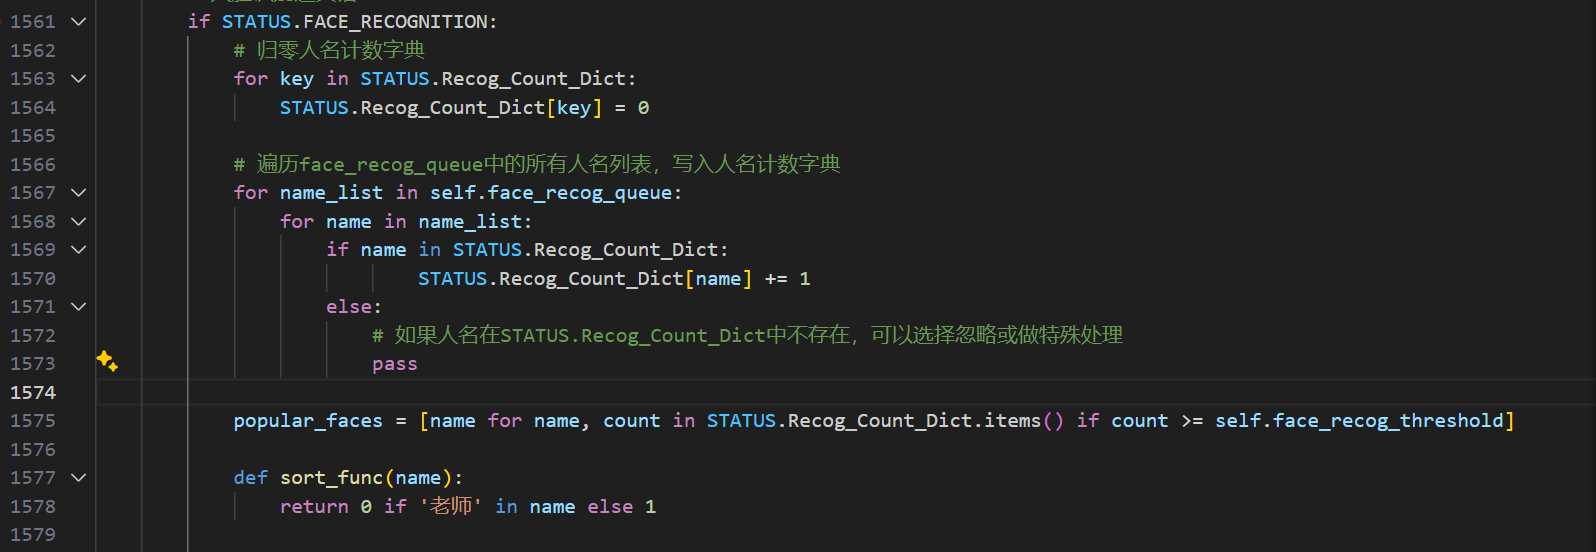
\includegraphics[width=0.7\linewidth]{screenshot002}
		\label{fig:screenshot002}
	\end{figure}
	没看懂这里的self.face\_recog\_queue和STATUS.Recog\_Count\_Dict应该是存的什么东西,谁在维护,哪里进行人脸识别
	
\end{itemize}	
\end{document}
